\chapter{Clase 2: Modelo de regresión lineal simple}

\section{De la asociación a la regresión}

Al estudiar dos variables cuantitativas preguntamos si están relacionadas, cuál parece ser la forma y el grado de esa relación, y si una variable puede ayudar a predecir la otra. El análisis de correlación resume la asociación; la regresión describe una forma para el valor medio de una variable respuesta $Y$ en función de una variable predictora $X$.

En esta clase retomamos el ejemplo de las calificaciones de Matemáticas y Cálculo presentado en la Clase 1. La nube de puntos muestra una tendencia creciente, aunque las observaciones no caen exactamente sobre una recta. Para representar esa variación introducimos un modelo probabilístico.

\section{Modelo lineal con error aleatorio}

La parte sistemática del modelo es una función lineal de $X$. Para una observación con valor predictor $x$, su respuesta promedio se representa por
\[
\mathbb{E}(Y\mid X=x)=\alpha+\beta x,
\]
donde $\alpha$ es la ordenada al origen y $\beta$ es la pendiente de la recta de medias. La respuesta individual puede apartarse de ese promedio; por eso se incorpora un error aleatorio $\varepsilon$:
\[
Y=\alpha+\beta X+\varepsilon.
\]
Así, $\alpha+\beta x$ describe el nivel medio de la respuesta cuando $X=x$, mientras que $\varepsilon$ representa la desviación de una observación particular respecto a ese promedio.

\begin{figure}[H]
\centering
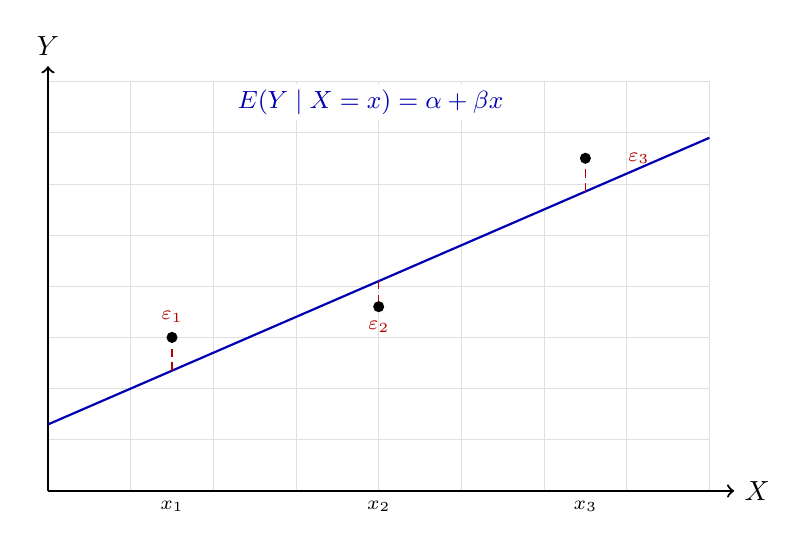
\begin{tikzpicture}[x=0.105cm,y=0.065cm]
    \draw[step=10,gray!25,very thin] (0,30) grid (80,110);
    \draw[->,thick] (0,30) -- (83,30) node[right] {$X$};
    \draw[->,thick] (0,30) -- (0,113) node[above] {$Y$};
    \draw[blue!70!black,thick] (0,43) -- (80,99);
    \node[blue!70!black,fill=white,inner sep=2pt,font=\small] at (39,106)
        {$\mathbb{E}(Y\mid X=x)=\alpha+\beta x$};
    \draw[densely dashed,red!70!black] (15,53.5) -- (15,60);
    \draw[densely dashed,red!70!black] (40,71) -- (40,66);
    \draw[densely dashed,red!70!black] (65,88.5) -- (65,95);
    \fill[black] (15,60) circle (2pt);
    \fill[black] (40,66) circle (2pt);
    \fill[black] (65,95) circle (2pt);
    \node[font=\scriptsize,red!70!black,above] at (15,61) {$\varepsilon_1$};
    \node[font=\scriptsize,red!70!black,below] at (40,65) {$\varepsilon_2$};
    \node[font=\scriptsize,red!70!black,right] at (69,95) {$\varepsilon_3$};
    \node[below,font=\scriptsize] at (15,30) {$x_1$};
    \node[below,font=\scriptsize] at (40,30) {$x_2$};
    \node[below,font=\scriptsize] at (65,30) {$x_3$};
\end{tikzpicture}
\caption{Esquema del modelo: las respuestas observadas se desvían de la recta de medias por el error aleatorio.}
\label{fig:modelo-lineal-error}
\end{figure}

\subsection{Supuestos sobre el error}

Para el modelo clásico de regresión lineal simple se consideran los siguientes supuestos sobre los errores:

\begin{itemize}
    \item los errores de observaciones distintas son independientes;
    \item su media es cero: $\mathbb{E}(\varepsilon_i)=0$;
    \item tienen una varianza común $\operatorname{Var}(\varepsilon_i)=\sigma^2$;
    \item tienen distribución normal.
\end{itemize}

En particular, el supuesto de media cero hace que la recta $\alpha+\beta x$ coincida con la respuesta promedio para cada valor de $x$. La varianza común indica que la dispersión alrededor de la recta se supone similar a lo largo del rango de $X$. Estos supuestos describen el modelo y no garantizan que se cumplan para cualquier conjunto de datos.

\section{La recta estimada y los residuos}

En una muestra se desconocen los parámetros $\alpha$ y $\beta$. Se estiman con valores $a$ y $b$, y se obtiene la recta ajustada
\[
\widehat{y}=a+bx.
\]
Para la observación $i$, el valor estimado es $\widehat{y}_i=a+bx_i$. La diferencia entre la respuesta observada y la estimada se llama \textbf{residuo}:
\[
e_i=y_i-\widehat{y}_i.
\]
El error $\varepsilon_i$ del modelo es una cantidad aleatoria no observada; el residuo $e_i$ se calcula después de ajustar la recta y sirve para describir la diferencia en los datos.

\subsection{Criterio de mínimos cuadrados}

Una recta puede quedar por encima de algunas observaciones y por debajo de otras. La suma simple de las diferencias con signo puede cancelarse; por eso se elige la recta minimizando la suma de los cuadrados de los residuos:
\[
S(a,b)=\sum_{i=1}^{n}e_i^2
=\sum_{i=1}^{n}\bigl(y_i-(a+bx_i)\bigr)^2.
\]
El \textbf{método de mínimos cuadrados} escoge $a$ y $b$ de modo que $S(a,b)$ sea lo menor posible. Las distancias consideradas son verticales, pues para cada $x_i$ se compara $y_i$ con el valor de la recta en ese mismo punto.

\begin{figure}[H]
\centering
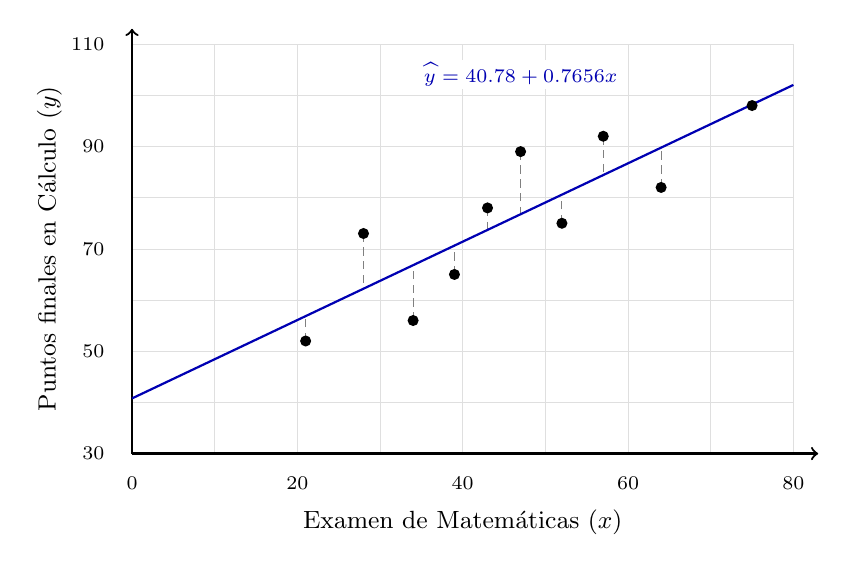
\begin{tikzpicture}[x=0.105cm,y=0.065cm]
    \draw[step=10,gray!25,very thin] (0,30) grid (80,110);
    \draw[->,thick] (0,30) -- (83,30);
    \draw[->,thick] (0,30) -- (0,113);
    \foreach \x in {0,20,40,60,80} {
        \node[below=2pt,font=\scriptsize] at (\x,28.5) {\x};
    }
    \foreach \y in {30,50,70,90,110} {
        \node[left=2pt,font=\scriptsize] at (-1.5,\y) {\y};
    }
    \node[below=14pt,font=\small] at (40,28.5) {Examen de Matemáticas ($x$)};
    \node[rotate=90,font=\small] at (-10,70) {Puntos finales en Cálculo ($y$)};
    \draw[gray,densely dashed] (39,65) -- (39,70.64);
    \draw[gray,densely dashed] (43,78) -- (43,73.70);
    \draw[gray,densely dashed] (21,52) -- (21,56.86);
    \draw[gray,densely dashed] (64,82) -- (64,89.78);
    \draw[gray,densely dashed] (57,92) -- (57,84.42);
    \draw[gray,densely dashed] (47,89) -- (47,76.77);
    \draw[gray,densely dashed] (28,73) -- (28,62.22);
    \draw[gray,densely dashed] (75,98) -- (75,98.20);
    \draw[gray,densely dashed] (34,56) -- (34,66.81);
    \draw[gray,densely dashed] (52,75) -- (52,80.59);
    \draw[blue!70!black,thick] (0,40.78) -- (80,102.03);
    \node[blue!70!black,fill=white,inner sep=1pt,font=\scriptsize] at (47,104) {$\widehat y=40.78+0.7656x$};
    \foreach \x/\y in {39/65,43/78,21/52,64/82,57/92,47/89,28/73,75/98,34/56,52/75} {
        \fill[black] (\x,\y) circle (2pt);
    }
\end{tikzpicture}
\caption{Recta ajustada al ejemplo y distancias verticales entre cada dato y su valor estimado.}
\label{fig:minimos-cuadrados}
\end{figure}

\section{Fórmulas de la recta de mínimos cuadrados}

Sin desarrollar aquí el cálculo diferencial, las fórmulas para los estimadores de mínimos cuadrados son
\[
b=\frac{s_{XY}}{s_X^2},\qquad a=\bar{y}-b\bar{x},
\]
donde $\bar{x}$ y $\bar{y}$ son los promedios muestrales, $s_{XY}$ es la covarianza muestral entre $X$ y $Y$, y $s_X^2$ es la varianza muestral de $X$. De manera equivalente, si se definen las sumas centradas
\[
C_{XY}=\sum_{i=1}^n(x_i-\bar{x})(y_i-\bar{y}),\qquad
C_{XX}=\sum_{i=1}^n(x_i-\bar{x})^2,
\]
entonces
\[
b=\frac{C_{XY}}{C_{XX}},\qquad a=\bar{y}-b\bar{x}.
\]
El parámetro $b$ es la pendiente estimada: señala cuánto cambia $\widehat y$ cuando $x$ aumenta una unidad. El valor $a$ es la ordenada al origen de la recta estimada.

\subsection{Cálculo con las calificaciones del ejemplo}

La tabla de la Clase 1 contiene los diez pares observados. Para calcular la recta se necesitan también las sumas de cuadrados y productos:

\begin{table}[H]
\centering
\small
\renewcommand{\arraystretch}{1.08}
\begin{tabular}{|r|r|r|r|r|}
\hline
\textbf{Estudiante} & $x_i$ & $y_i$ & $x_i^2$ & $x_iy_i$ \\ \hline
1 & 39 & 65 & 1521 & 2535 \\ \hline
2 & 43 & 78 & 1849 & 3354 \\ \hline
3 & 21 & 52 & 441 & 1092 \\ \hline
4 & 64 & 82 & 4096 & 5248 \\ \hline
5 & 57 & 92 & 3249 & 5244 \\ \hline
6 & 47 & 89 & 2209 & 4183 \\ \hline
7 & 28 & 73 & 784 & 2044 \\ \hline
8 & 75 & 98 & 5625 & 7350 \\ \hline
9 & 34 & 56 & 1156 & 1904 \\ \hline
10 & 52 & 75 & 2704 & 3900 \\ \hline
\textbf{Suma} & \textbf{460} & \textbf{760} & \textbf{23634} & \textbf{36854} \\ \hline
\end{tabular}
\caption{Cálculos auxiliares para ajustar la recta a los datos de calificaciones.}
\label{tab:calculos-regresion-simple}
\end{table}

De la tabla se obtienen $\bar{x}=460/10=46$ y $\bar{y}=760/10=76$. Por tanto,
\begin{align*}
C_{XY}&=\sum x_iy_i-n\bar{x}\bar{y}
=36854-10(46)(76)=1894,\\
C_{XX}&=\sum x_i^2-n\bar{x}^{\,2}
=23634-10(46)^2=2474.
\end{align*}
Así, la pendiente y la ordenada al origen son
\begin{align*}
b&=\frac{1894}{2474}\approx0.7656,\\
a&=76-(0.7656)(46)\approx40.78.
\end{align*}
La recta estimada para estos datos es
\[
\widehat y=40.78+0.7656x.
\]
Según esta recta, por cada punto adicional en el examen de Matemáticas, el valor estimado de los puntos finales en Cálculo aumenta aproximadamente $0.77$ puntos. La interpretación corresponde a la recta ajustada y no significa que cada estudiante siga exactamente esa relación.

\section{Covarianza y signo de la pendiente}

La covarianza resume cómo varían conjuntamente las observaciones de $X$ y $Y$. Una definición descriptiva es
\[
S_{XY}=\frac{1}{n}\sum_{i=1}^{n}(x_i-\bar{x})(y_i-\bar{y}).
\]
También es usual definir la covarianza muestral con denominador $n-1$. En la fórmula de la pendiente se usan covarianza y varianza con el mismo denominador; por ello, el factor común se cancela y se obtiene $b=C_{XY}/C_{XX}$ en cualquiera de las dos convenciones.

Cada producto $(x_i-\bar{x})(y_i-\bar{y})$ es positivo cuando $x_i$ e $y_i$ están ambos por encima de sus promedios o ambos por debajo; es negativo cuando uno está por encima y el otro por debajo. El signo conjunto que predomina determina el signo de la covarianza. Como $C_{XX}>0$ para una variable $X$ no constante, la pendiente $b=C_{XY}/C_{XX}$ tiene el mismo signo que la covarianza:

\begin{itemize}
    \item si $b>0$, la relación lineal estimada es directa: valores mayores de $X$ se asocian con valores mayores de $Y$;
    \item si $b<0$, la relación lineal estimada es inversa: valores mayores de $X$ se asocian con valores menores de $Y$.
\end{itemize}

\begin{figure}[H]
\centering
\begin{tikzpicture}[scale=0.78]
    \foreach \shift/\title in {0/{Covarianza positiva},6.2/{Covarianza negativa},12.4/{Covarianza casi nula}} {
        \begin{scope}[xshift=\shift cm]
            \draw[->,gray] (-2.7,0) -- (2.7,0);
            \draw[->,gray] (0,-2.7) -- (0,2.7);
            \node[font=\scriptsize,below right] at (1.9,-0.12) {$x-\bar{x}$};
            \node[font=\scriptsize,above left] at (0,2.7) {$y-\bar{y}$};
            \node[font=\small] at (0,-3.35) {\title};
        \end{scope}
    }
    \begin{scope}
        \foreach \x/\y in {-2/-2,-1/-1.5,-1.5/-0.8,-0.8/-1,0.8/0.8,1/1.5,1.5/0.8,2/2} {\fill[blue!70!black] (\x,\y) circle (2.2pt);}
        \node[font=\scriptsize] at (1.75,2.5) {$S_{XY}>0$};
    \end{scope}
    \begin{scope}[xshift=6.2cm]
        \foreach \x/\y in {-2/2,-1/1.5,-1.5/0.8,-0.8/1,0.8/-0.8,1/-1.5,1.5/-0.8,2/-2} {\fill[blue!70!black] (\x,\y) circle (2.2pt);}
        \node[font=\scriptsize] at (1.75,2.5) {$S_{XY}<0$};
    \end{scope}
    \begin{scope}[xshift=12.4cm]
        \foreach \x/\y in {-2/1,-1/-2,-1.5/0.4,-0.8/1.6,0.8/-1.6,1.5/-0.4,1/2,2/-1} {\fill[blue!70!black] (\x,\y) circle (2.2pt);}
        \node[font=\scriptsize] at (1.75,2.5) {$S_{XY}\approx0$};
    \end{scope}
\end{tikzpicture}
\caption{Patrones esquemáticos de los productos centrados y el signo de la covarianza.}
\label{fig:signo-covarianza-regresion}
\end{figure}

En el ejemplo de calificaciones, $C_{XY}=1894>0$ y $C_{XX}=2474>0$, así que $b>0$. Esto concuerda con la tendencia creciente observada en el diagrama de dispersión.

\section{Diagnóstico del modelo mediante residuos}

Las conclusiones de una regresión son confiables cuando los supuestos del modelo son razonables para los datos. Además de revisar el contexto y la forma de la nube de puntos, podemos estudiar los residuos. En el ejemplo de las calificaciones, la recta ajustada es $\widehat{y}=40.78+0.7656x$; la siguiente tabla muestra los valores estimados y los residuos, redondeados a dos decimales.

\begin{table}[H]
\centering
\small
\renewcommand{\arraystretch}{1.08}
\begin{tabular}{|r|r|r|r|}
\hline
\textbf{Estudiante} & $y_i$ & $\widehat{y}_i$ & $e_i=y_i-\widehat{y}_i$ \\ \hline
1 & 65 & 70.64 & $-5.64$ \\ \hline
2 & 78 & 73.70 & 4.30 \\ \hline
3 & 52 & 56.86 & $-4.86$ \\ \hline
4 & 82 & 89.78 & $-7.78$ \\ \hline
5 & 92 & 84.42 & 7.58 \\ \hline
6 & 89 & 76.77 & 12.23 \\ \hline
7 & 73 & 62.22 & 10.78 \\ \hline
8 & 98 & 98.20 & $-0.20$ \\ \hline
9 & 56 & 66.81 & $-10.81$ \\ \hline
10 & 75 & 80.59 & $-5.59$ \\ \hline
\end{tabular}
\caption{Respuestas estimadas y residuos para los diez estudiantes.}
\label{tab:residuos-calificaciones}
\end{table}

En mínimos cuadrados con intercepto, la suma de los residuos es cero (salvo diferencias de redondeo en la tabla), de modo que su media muestral es cero. Para buscar patrones que indiquen problemas con los supuestos se utilizan varias gráficas:

\begin{itemize}
    \item \textbf{Residuos contra orden de observación:} se revisa si aparecen tendencias, ciclos o agrupamientos. Un patrón puede ser indicio de que los errores no son independientes.
    \item \textbf{Residuos contra valores ajustados:} se espera una nube aleatoria alrededor de cero y con dispersión aproximadamente constante. Una curva puede indicar que la relación no es lineal; una forma de embudo puede indicar que la varianza cambia con el ajuste.
    \item \textbf{Gráfico Q--Q:} compara los residuos ordenados con los cuantiles teóricos de una distribución normal. Si la normalidad es plausible, los puntos suelen aproximarse a una línea creciente.
\end{itemize}

\begin{figure}[H]
\centering
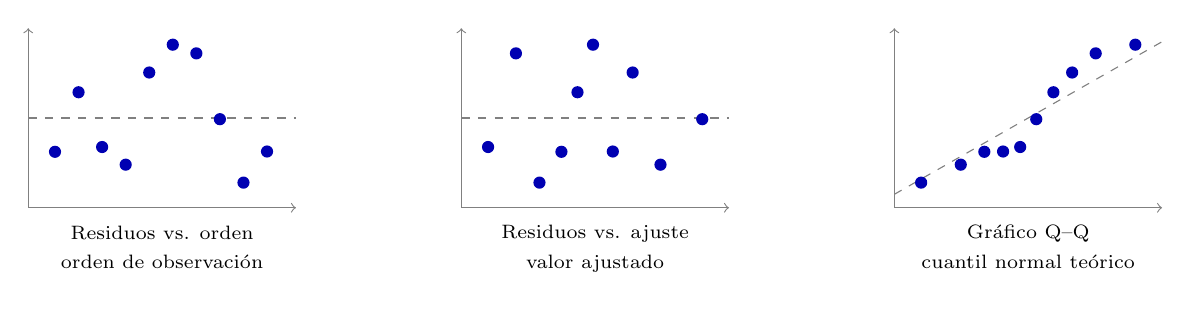
\begin{tikzpicture}[x=0.68cm,y=0.38cm,font=\scriptsize]
    % Residuos contra el orden de observación
    \begin{scope}
        \draw[->,gray] (0,-3) -- (5,-3);
        \draw[->,gray] (0,-3) -- (0,3);
        \draw[gray,dashed] (0,0) -- (5,0);
        \foreach \x/\e in {0.5/-1.13,0.94/0.86,1.38/-0.97,1.82/-1.56,2.26/1.52,2.70/2.45,3.14/2.16,3.58/-0.04,4.02/-2.16,4.46/-1.12} {\fill[blue!70!black] (\x,\e) circle (2.2pt);}
        \node[align=center] at (2.5,-3.85) {Residuos vs. orden};
        \node[below] at (2.5,-4.25) {orden de observación};
    \end{scope}
    % Residuos contra valores ajustados
    \begin{scope}[xshift=5.5cm]
        \draw[->,gray] (0,-3) -- (5,-3);
        \draw[->,gray] (0,-3) -- (0,3);
        \draw[gray,dashed] (0,0) -- (5,0);
        \foreach \x/\e in {1.87/-1.13,2.17/0.86,0.50/-0.97,3.72/-1.56,3.20/1.52,2.46/2.45,1.02/2.16,4.50/-0.04,1.46/-2.16,2.83/-1.12} {\fill[blue!70!black] (\x,\e) circle (2.2pt);}
        \node[align=center] at (2.5,-3.85) {Residuos vs. ajuste};
        \node[below] at (2.5,-4.25) {valor ajustado};
    \end{scope}
    % Gráfico Q--Q con los residuos ordenados
    \begin{scope}[xshift=11cm]
        \draw[->,gray] (0,-3) -- (5,-3);
        \draw[->,gray] (0,-3) -- (0,3);
        \draw[gray,dashed] (0,-2.55) -- (5,2.55);
        \foreach \x/\e in {0.50/-2.16,1.24/-1.56,1.68/-1.13,2.03/-1.12,2.35/-0.97,2.65/-0.04,2.97/0.86,3.32/1.52,3.76/2.16,4.50/2.45} {\fill[blue!70!black] (\x,\e) circle (2.2pt);}
        \node[align=center] at (2.5,-3.85) {Gráfico Q--Q};
        \node[below] at (2.5,-4.25) {cuantil normal teórico};
    \end{scope}
\end{tikzpicture}
\caption{Esquemas de diagnóstico residual. En los dos primeros paneles se representan los residuos del ejemplo; en el Q--Q, su comparación con cuantiles normales aproximados.}
\label{fig:diagnostico-residuos}
\end{figure}

En el gráfico Q--Q de este ejemplo no se aprecia una desviación marcada de la forma lineal. Esto no demuestra que los errores sean normales; con solo diez observaciones, el diagnóstico tiene alcance limitado.

Estas gráficas son herramientas de diagnóstico, no pruebas concluyentes. En particular, con una muestra pequeña conviene interpretarlas con cautela y junto con el conocimiento del problema.

\section{Correlación y tipos de dependencia}

El análisis de correlación se ocupa de medir la intensidad de la asociación entre dos variables; en este contexto nos interesa especialmente la asociación lineal. La covarianza vista antes ayuda a reconocer el sentido de la variación conjunta, mientras que el análisis de regresión busca representar la relación y estimar la respuesta a partir de la variable predictora.

Las relaciones entre $X$ e $Y$ pueden adoptar distintas formas. En una relación estadística, para un mismo valor de $X$ puede haber variación en $Y$; la nube puede no mostrar un patrón claro, o mostrar una tendencia lineal o curvilínea. En una dependencia funcional, en cambio, cada valor de $X$ determina exactamente un valor de $Y$, por lo que todos los puntos quedan sobre una curva.

\begin{figure}[H]
\centering
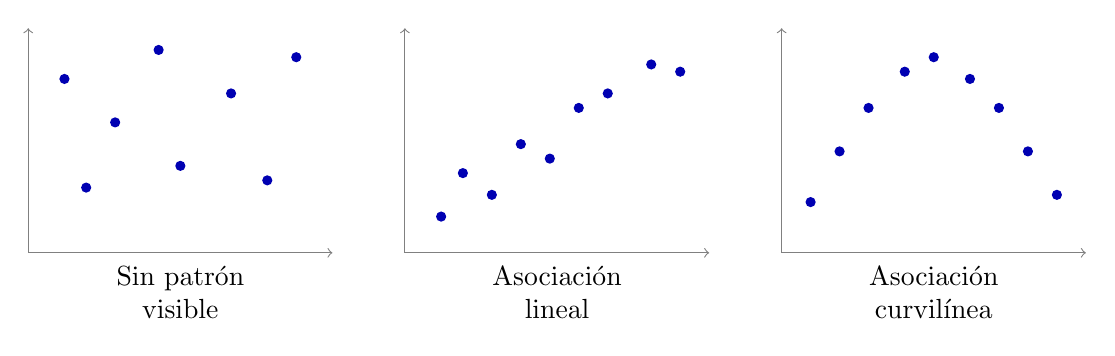
\begin{tikzpicture}[scale=0.92]
    % Sin patrón evidente
    \begin{scope}
        \draw[->,gray] (0,0) -- (4.2,0);
        \draw[->,gray] (0,0) -- (0,3.1);
        \foreach \x/\y in {0.5/2.4,0.8/0.9,1.2/1.8,1.8/2.8,2.1/1.2,2.8/2.2,3.3/1.0,3.7/2.7} {\fill[blue!70!black] (\x,\y) circle (2pt);}
        \node[align=center] at (2.1,-0.55) {Sin patrón\\visible};
    \end{scope}
    % Asociación estadística lineal
    \begin{scope}[xshift=5.2cm]
        \draw[->,gray] (0,0) -- (4.2,0);
        \draw[->,gray] (0,0) -- (0,3.1);
        \foreach \x/\y in {0.5/0.5,0.8/1.1,1.2/0.8,1.6/1.5,2.0/1.3,2.4/2.0,2.8/2.2,3.4/2.6,3.8/2.5} {\fill[blue!70!black] (\x,\y) circle (2pt);}
        \node[align=center] at (2.1,-0.55) {Asociación\\lineal};
    \end{scope}
    % Asociación estadística curvilínea
    \begin{scope}[xshift=10.4cm]
        \draw[->,gray] (0,0) -- (4.2,0);
        \draw[->,gray] (0,0) -- (0,3.1);
        \foreach \x/\y in {0.4/0.7,0.8/1.4,1.2/2.0,1.7/2.5,2.1/2.7,2.6/2.4,3.0/2.0,3.4/1.4,3.8/0.8} {\fill[blue!70!black] (\x,\y) circle (2pt);}
        \node[align=center] at (2.1,-0.55) {Asociación\\curvilínea};
    \end{scope}
\end{tikzpicture}
\caption{Ejemplos esquemáticos de ausencia de patrón visible y de asociaciones estadísticas lineal y curvilínea.}
\label{fig:dependencia-estadistica}
\end{figure}

\begin{figure}[H]
\centering
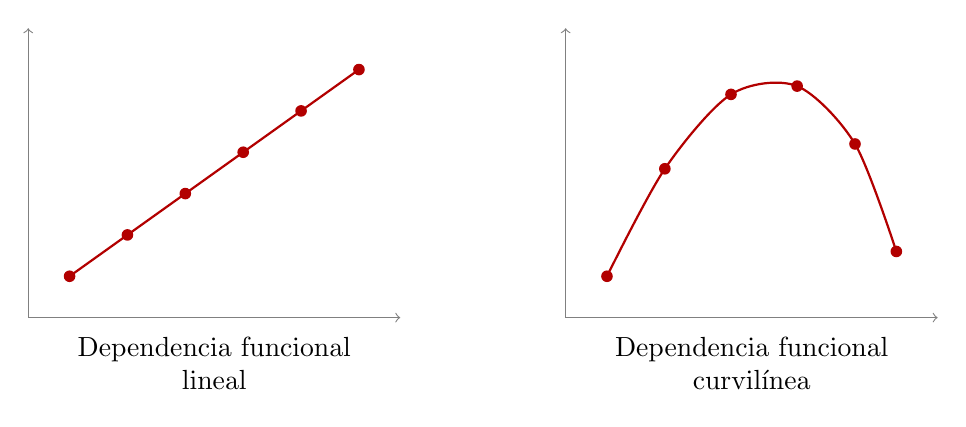
\begin{tikzpicture}[scale=1.05]
    % Dependencia lineal funcional
    \begin{scope}[xshift=1cm]
        \draw[->,gray] (0,0) -- (4.5,0);
        \draw[->,gray] (0,0) -- (0,3.5);
        \draw[red!70!black,thick] (0.5,0.5) -- (4,3.0);
        \foreach \x/\y in {0.5/0.5,1.2/1.0,1.9/1.5,2.6/2.0,3.3/2.5,4/3.0} {\fill[red!70!black] (\x,\y) circle (2pt);}
        \node[align=center] at (2.25,-0.55) {Dependencia funcional\\lineal};
    \end{scope}
    % Dependencia curvilínea funcional
    \begin{scope}[xshift=7.5cm]
        \draw[->,gray] (0,0) -- (4.5,0);
        \draw[->,gray] (0,0) -- (0,3.5);
        \draw[red!70!black,thick] plot[smooth] coordinates {(0.5,0.5) (1.2,1.8) (2.0,2.7) (2.8,2.8) (3.5,2.1) (4,0.8)};
        \foreach \x/\y in {0.5/0.5,1.2/1.8,2.0/2.7,2.8/2.8,3.5/2.1,4/0.8} {\fill[red!70!black] (\x,\y) circle (2pt);}
        \node[align=center] at (2.25,-0.55) {Dependencia funcional\\curvilínea};
    \end{scope}
\end{tikzpicture}
\caption{En una dependencia funcional, las observaciones siguen exactamente una relación lineal o curvilínea.}
\label{fig:dependencia-funcional}
\end{figure}

\section{Ecuaciones y tipos de regresión}

A la función que describe la respuesta en términos de la variable predictora se le llama \textbf{ecuación de regresión}. Algunos ejemplos son
\[
\widehat{y}=a+bx
\qquad\text{y}\qquad
\widehat{y}=a+bx+cx^2.
\]
La primera representa una recta; la segunda, una relación parabólica. También existen modelos curvilíneos de tipo exponencial o potencial. En una regresión lineal simple se utiliza una sola variable predictora y la ecuación es lineal en sus parámetros. Cuando se incluyen varias variables predictoras para una sola respuesta, se habla de regresión múltiple.

La forma de la nube de puntos ayuda a decidir qué tipo de relación podría describir los datos. En esta clase nos hemos concentrado en el caso simple lineal y en los conceptos de diagnóstico presentados en las páginas indicadas.


\clearpage
\section{Supuestos que fundamentan la inferencia}

Los supuestos ya presentados pueden precisarse para interpretar el modelo y realizar inferencias sobre sus parámetros. En el modelo clásico de regresión lineal simple se considera que:

\begin{enumerate}
    \item los valores de $X$ se fijan mediante el diseño del estudio. En otras aplicaciones, $X$ puede ser aleatoria; el análisis se formula entonces condicionando en los valores observados de $X$;
    \item $X$ se mide con error despreciable;
    \item para cada valor de $X$, la distribución condicional de $Y$ es normal cuando se requieren los procedimientos usuales de inferencia;
    \item la varianza condicional de $Y$ es constante para todos los valores de $X$;
    \item la media condicional de $Y$ sigue una función lineal, $\mathbb{E}(Y\mid X=x)=\alpha+\beta x$;
    \item las observaciones son independientes entre sí, condicionalmente a los valores de $X$.
\end{enumerate}

Estos supuestos se resumen escribiendo, para cada observación,
\[
Y_i=\alpha+\beta x_i+\varepsilon_i,
\]
donde $\varepsilon_i=Y_i-\mathbb{E}(Y_i\mid X=x_i)$ es la desviación respecto de la media condicional. En particular,
\[
\mathbb{E}(\varepsilon_i\mid X)=0,\qquad
\operatorname{Var}(\varepsilon_i\mid X)=\sigma^2,
\]
y, bajo el supuesto de normalidad, los errores condicionales tienen distribución normal. Un recordatorio de cuatro supuestos para la inferencia es la sigla \textbf{LINI}: linealidad, independencia, normalidad e igualdad de varianzas.

\subsection{Significado de los coeficientes}

El parámetro $\alpha$ es la ordenada al origen de la recta de medias: representa la respuesta promedio cuando $X=0$. Esta interpretación solo es sustantiva si $X=0$ tiene sentido en el problema y está dentro de un rango pertinente. El parámetro $\beta$ es la pendiente: por cada unidad que aumenta $X$, la media de $Y$ cambia en $\beta$ unidades. En la muestra, los estimadores $a$ y $b$ dan la recta ajustada $\widehat y=a+bx$ y estiman, respectivamente, $\alpha$ y $\beta$.

\section{Representatividad de la recta y variación residual}

La recta de mínimos cuadrados resume la tendencia media de los datos, pero ser la mejor recta posible según el criterio de mínimos cuadrados no garantiza que represente bien la nube de puntos. Para describir la distancia de las observaciones a la recta se utilizan los residuos $e_i=y_i-\widehat y_i$. Una medida descriptiva de dispersión residual es
\[
S_e^2=\frac{1}{n}\sum_{i=1}^{n}e_i^2=\frac{SSE}{n}.
\]
Valores pequeños indican que, en promedio cuadrático, los datos están cerca de la recta. En inferencia de regresión también es usual estimar la varianza del error mediante $SSE/(n-2)$, pues se estiman dos coeficientes.

\subsection{Descomposición de la variación}

La variación total observada en la respuesta se mide con
\[
SST=S_{yy}=\sum_{i=1}^{n}(y_i-\bar y)^2.
\]
En una regresión lineal ajustada por mínimos cuadrados con intercepto, esta variación se descompone en la parte explicada por la recta y la parte residual:
\begin{align*}
SST&=SSR+SSE,\\
SSR&=\sum_{i=1}^{n}(\widehat y_i-\bar y)^2,\\
SSE&=\sum_{i=1}^{n}(y_i-\widehat y_i)^2=\sum_{i=1}^{n}e_i^2.
\end{align*}
La igualdad expresa que la variación total alrededor de $\bar y$ es la suma de la variación de los valores ajustados alrededor de $\bar y$ y la variación que queda en los residuos.

Para una observación particular, la desviación total puede separarse en una parte asociada con el ajuste y un residuo:
\[
y_i-\bar y=(\widehat y_i-\bar y)+(y_i-\widehat y_i).
\]
La figura muestra esta relación para el quinto estudiante del ejemplo, para quien $y_i=92$, $\widehat y_i=84.42$ y $\bar y=76$.

\begin{figure}[H]
\centering
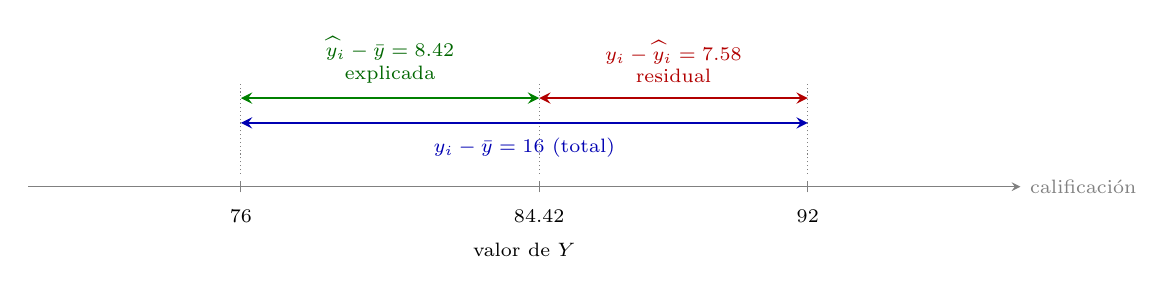
\begin{tikzpicture}[x=0.45cm,y=0.9cm,>=stealth,font=\scriptsize]
    % Para el estudiante 5: media 76, ajuste 84.42 y respuesta observada 92.
    \draw[->,gray] (70,0) -- (98,0) node[right] {calificación};
    \foreach \x/\etiqueta in {76/76,84.42/84.42,92/92} {
        \draw[gray] (\x,-0.08) -- (\x,0.08);
        \node[below=3pt] at (\x,-0.08) {\etiqueta};
    }
    \node[below=17pt,align=center] at (84,0) {valor de $Y$};

    \draw[densely dotted,gray] (76,0.18) -- (76,1.45);
    \draw[densely dotted,gray] (84.42,0.18) -- (84.42,1.45);
    \draw[densely dotted,gray] (92,0.18) -- (92,1.45);

    \draw[<->,thick,green!50!black] (76,1.25) -- (84.42,1.25);
    \node[above=2pt,align=center,text=green!40!black] at (80.21,1.25)
        {$\widehat y_i-\bar y=8.42$\\explicada};
    \draw[<->,thick,red!70!black] (84.42,1.25) -- (92,1.25);
    \node[above=2pt,align=center,text=red!70!black] at (88.21,1.25)
        {$y_i-\widehat y_i=7.58$\\residual};

    \draw[<->,thick,blue!70!black] (76,0.9) -- (92,0.9);
    \node[below=2pt,align=center,text=blue!70!black] at (84,0.9)
        {$y_i-\bar y=16$ (total)};
\end{tikzpicture}
\caption{Descomposición de la desviación de una observación en una parte explicada por el ajuste y un residuo.}
\label{fig:descomposicion-variacion}
\end{figure}

En el ejemplo de las calificaciones, las sumas centradas anteriores son $S_{xx}=C_{XX}=2474$ y $S_{xy}=C_{XY}=1894$. Como $b=S_{xy}/S_{xx}$, se obtiene
\begin{align*}
SSR&=b^2S_{xx}=\frac{S_{xy}^2}{S_{xx}}\approx1449.97,\\
SSE&=SST-SSR.
\end{align*}
Además, $S_{yy}=\sum y_i^2-n\bar y^{\,2}=59816-10(76)^2=2056$, por lo que $SSE\approx606.03$. Se verifica así que $2056\approx1449.97+606.03$.

\section{Coeficiente de determinación}

El \textbf{coeficiente de determinación}, denotado por $R^2$, mide la proporción de la variación muestral de $Y$ explicada por la recta de regresión:
\begin{align*}
R^2&=\frac{SSR}{SST}
=1-\frac{SSE}{SST}\\
&=\frac{S_{xy}^2}{S_{xx}S_{yy}}
=r^2,
\end{align*}
donde $r$ es el coeficiente de correlación lineal muestral. La igualdad $R^2=r^2$ se cumple en la regresión lineal simple con intercepto. Aquí $S_{xx}=\sum_i(x_i-\bar x)^2$, $S_{xy}=\sum_i(x_i-\bar x)(y_i-\bar y)$ y $S_{yy}=\sum_i(y_i-\bar y)^2$.

Con intercepto, $0\leq R^2\leq1$. El porcentaje de variación no explicado por la recta es
\[
\frac{SSE}{SST}\cdot100\%=(1-R^2)\cdot100\%.
\]
Para las calificaciones, $R^2\approx1449.97/2056\approx0.7052$. Así, la recta explica aproximadamente el $70.52\%$ de la variación muestral de los puntos de Cálculo; el $29.48\%$ restante queda en los residuos. Esta proporción describe el ajuste lineal en estos datos y no implica por sí misma una relación causal.

Si $R^2=1$, todos los puntos quedan sobre la recta ajustada y existe dependencia lineal funcional en la muestra. Valores cercanos a uno indican que la recta explica una fracción grande de la variación observada. Si $R^2=0$, la recta no explica variación lineal respecto de la media de $Y$; esto no descarta que exista una relación no lineal entre las variables.